% to compile: Shift+Alt+F1
\documentclass[a4paper,11pt]{article}%,twocolumn
%% packages

\usepackage{blindtext} % needed for creating dummy text passages
%\usepackage{ngerman} % needed for German default language
\usepackage{amsmath} % needed for command eqref
\usepackage{amssymb} % needed for math fonts
\usepackage[colorlinks=true,breaklinks]{hyperref} % needed for creating hyperlinks in the document, the option colorlinks=true gets rid of the awful boxes, breaklinks breaks lonkg links (list of figures), and ngerman sets everything for german as default hyperlinks language
\usepackage[hyphenbreaks]{breakurl} % ben�tigt f�r das Brechen von URLs in Literaturreferenzen, hyphenbreaks auch bei links, die �ber eine Seite gehen (mit hyphenation).
\usepackage{xcolor}
\definecolor{c1}{rgb}{0,0,1} % blue
\definecolor{c2}{rgb}{0,0.3,0.9} % light blue
\definecolor{c3}{rgb}{0.3,0,0.9} % red blue
\hypersetup{
    linkcolor={c1}, % internal links
    citecolor={c2}, % citations
    urlcolor={c3} % external links/urls
}
%\usepackage{cite} % needed for cite
\usepackage[square,authoryear]{natbib} % needed for cite and abbrvnat bibliography style
\usepackage[nottoc]{tocbibind} % needed for displaying bibliography and other in the table of contents
\usepackage{graphicx} % needed for \includegraphics 
\usepackage{longtable} % needed for long tables over pages
\usepackage{bigstrut} % needed for the command \bigstrut
\usepackage{enumerate} % needed for some options in enumerate
%\usepackage{todonotes} % needed for todos
\usepackage{makeidx} % needed for creating an index
\makeindex
\usepackage{gensymb}
%\usepackage{url}
\usepackage{xurl}
\usepackage{psfrag}
\usepackage{multirow}
\usepackage{subfigure}

\usepackage{algpseudocode}
\usepackage{float}
%\usepackage{minted}
\usepackage{tcolorbox}
\usepackage{menukeys}
\usepackage[
width=.8\textwidth,
justification=centering]{caption}
\usepackage{xcolor}
\usepackage{pstricks}
\usepackage{acronym}
%% page settings

\usepackage[top=20mm, bottom=20mm,left=20mm,right=20mm]{geometry} % needed for page border settings
\parindent=0mm % for space of first line of new text block
\sloppy % for writing with hyphenless justification (tries to)
\hyphenation{} % use hyphenation of tolerance parametershttp://www.jr-x.de/publikationen/latex/tipps/zeilenumbruch.html
\hyphenpenalty=10000
\exhyphenpenalty=10000
\usepackage{fancyhdr} % needed for head and foot options
%% my macros

%% Text fomats
\newcommand{\tbi}[1]{\textbf{\textit{#1}}}

% IEEE naming convention
%\renewcommand{\figurename}{Fig.}

% custom counter for shell scripts
\newcounter{shellcounter}
% \newcounter{myexample}% preamble
\newtcolorbox[
use counter=shellcounter,
number format=\Alph]{shell}[2][]{%
	colback=blue!5!white,
	colframe=blue!75!white,
	fonttitle=\bfseries,
	title= {\sc Shell \thetcbcounter}: #2,#1}


\newcounter{outputcounter}
\newtcolorbox[
use counter=outputcounter,
number format=\Roman]{result}[2][]{%
	colback=green!5!white,
	colframe=green!75!black,
	fonttitle=\bfseries,
	title= {\sc Result box \thetcbcounter}: #2,#1}


\begin{document}
\begin{titlepage}
\center % Center everything on the page

%-------------------------------------------------------------------------------------
%	HEADING SECTIONS
%------------------------------------------------------------------------------------
\textbf{\large Department of Electronic and Telecommunication Engineering}\\[0.5cm]
\textbf{\Large University of Moratuwa, Sri Lanka}\\[1cm]
\textbf{\large EN4603 - Digital IC Design}\\[2cm]

\includegraphics[width=0.3\textwidth]{figures/uomlogo}\\[2cm]

	
%-------------------------------------------------------------------------------------
%	TITLE SECTION
%------------------------------------------------------------------------------------
\textbf{\Huge Laboratory Experiment 1 \\RTL Synthesis }\\[0.2cm]
\textbf{\Large Laboratory Report}\\[3cm]


%----------------------------------------------------------------------------------------
%	MEMBERS SECTION
%----------------------------------------------------------------------------------------


\vfill

\textbf{\large Submitted by}\\[0.5cm]

\textbf{\large Submitted by}\\[2mm]
\begin{minipage}{0.3\textwidth}
	\begin{flushleft}
		{\large C.S.Pallikkonda}\\[2mm]
		{\large R.M.A.S.Rathnayake }\\[2mm]
		{\large B.P.Thalagala }\\[2mm]		
		
	\end{flushleft}
\end{minipage}
\hspace{2mm}
\begin{minipage}{0.2\textwidth}
	\begin{flushright}
		{\large 180441C }\\[2mm]
		{\large 180534N }\\[2mm]
		{\large 180631J }\\[2mm]

	\end{flushright}
\end{minipage}\\[1cm]

	
	
	
%----------------------------------------------------------------------------------------
%	DATE SECTION
%----------------------------------------------------------------------------------------

\textbf{\large Submitted on}\\[0.5cm]
\textbf{\Large \today} % Date, change the \today to a set date if you want to be precise

%----------------------------------------------------------------------------------------

\vfill % Fill the rest of the page with whitespace

\end{titlepage}

\pagebreak

\tableofcontents
\listoffigures
\listoftables
\section*{List of Abbreviations}
\addcontentsline{toc}{section}{List of Abbreviations}
\begin{acronym}
	\acro{asic}[ASIC]{Application Specific Integrated Circuit}
	\acro{atpg}[ATPG]{Automatic Test Pattern Generation}
	
	\acro{def}[DEF]{Design Exchange Format}
	\acro{dft}[DFT]{Design For Testability}
		
	\acro{gpdk}[GPDK]{Generic Process Design Kit}
		
	\acro{hdl}[HDL]{Hardware Description Language}
	
	\acro{ic}[IC]{Integrated Circuit}
		
	\acro{rtl}[RTL]{Register-Transfer Level}
	\acro{rx}[RX]{Receiver}
		
	\acro{tcl}[TCL]{Tool Command Language}
	\acro{tx}[TX]{Transmitter}
	
	\acro{uart}[UART]{Universal Asynchronous Receiver Transmitter}
	
\end{acronym}



\vfill

\textit{\textbf{Note:}}\\
\textit{All the materials related to the report can also be found at \url{https://github.com/bimalka98/Digital-IC-Design}}
\pagebreak


\pagebreak
\section{Introduction}

\subsection{Practical}
In this practical, we will be using \textit{Cadence Genus - Ver. 18.10 } to synthesize an example \ac{rtl} design, a transceiver. As inputs to Genus, we will provide

\begin{enumerate}
	\item Source Verilog files
	\item Technology libraries provided by the fabrication plant (here, $45~nm$ educational \ac{gpdk} given by Cadence) : {\tt (.lib, .lef, .tch)}
	
	\begin{itemize}
		\item Library Timing (.lib) files specify timing (cell delay, cell transition time, setup and hold time requirement) and power characteristics of standard cells. Slow and fast libraries 	characterize standard cells with maximum and minimum signal delays, which could occur from process variations.

		\item Tch files are binary files that accurately characterize library elements, that include  capacitance and resistance.
		
		\item Library Exchange Format (LEF) specify design rules, metal capacitances, layer information…etc.
	\end{itemize}
	
	\item Timing constraints
\end{enumerate}

and will obtain the synthesized netlist (Verilog files) and further timing constrains {\tt (.sdc)} as output. We will then analyze the area, timing and power of the synthesized design.

\pagebreak
\subsection{RTL Synthesis}

In the context of digital hardware design, \ac{rtl} synthesis is the process of converting an \ac{rtl} description of a digital circuit into an optimized gate-level design.\\

The \ac{rtl} description of a digital circuit is written in a \ac{hdl} such as Verilog or VHDL. It specifies the digital circuit in terms of the flow of digital signals between registers, and the logical operations that are performed on those signals as they are transferred between the registers.\\

During \ac{rtl} synthesis, an \ac{rtl} compiler reads the \ac{rtl} description of the digital circuit and generates an optimized gate-level representation of the circuit. This gate-level representation is a description of the digital circuit in terms of gates and interconnections between them. Figure \ref{fig:asic_flow} illustrates an overview of an \ac{rtl} synthesis flow.

\vfill

\begin{figure}[h]
	\centering
	\fbox{
		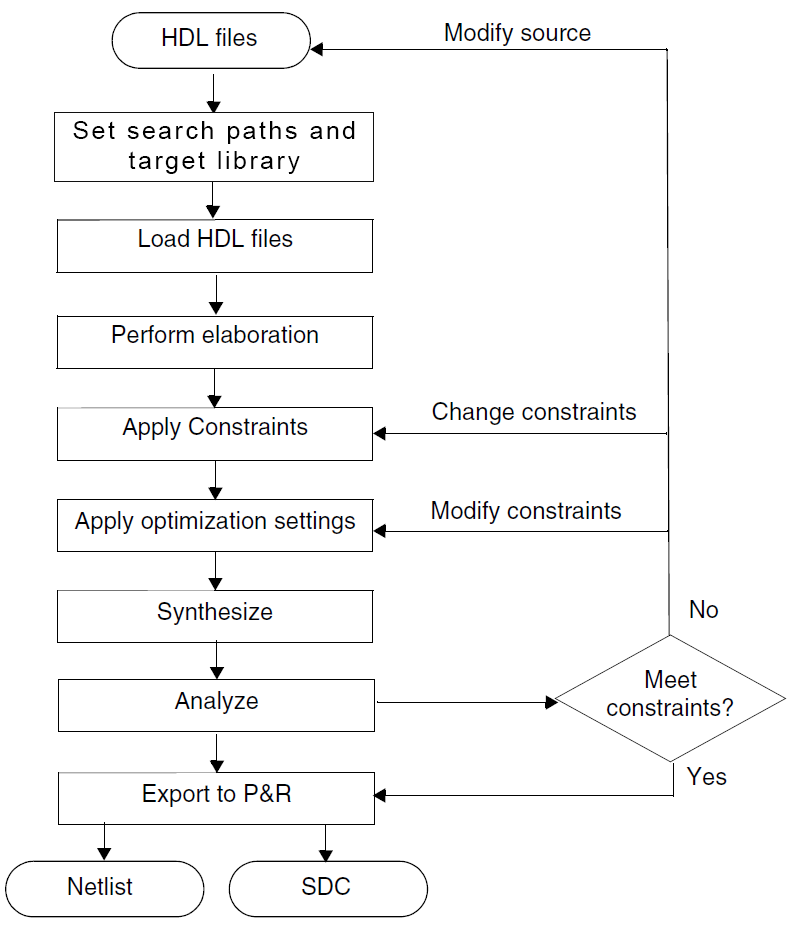
\includegraphics[width=0.8\linewidth]{figures/flow.PNG}
	}
	\caption{Overview of \ac{rtl} synthesis flow of Cadence Genus software\cite{genus_user_guide_2019}.}
	\label{fig:asic_flow}
\end{figure}

\pagebreak
\subsection{Associated Genus Commands}

\textbf{Note}: \textit{Genus is a \ac{tcl} based tool and therefore {\tt .tcl} scripts can be created to execute a series of commands instead of typing each command individually. The entire interface of Genus is accessible through \ac{tcl}, and true \ac{tcl} syntax and semantics are supported.}\\

Followings are the commands used in this lab, and the entire script could be executed once using a single {\tt .tcl} file. However, it was encouraged to execute the commands one-by-one in order to understand the process of synthesizing an \ac{rtl} design.
\vspace{2cm}
\begin{Verbatim}[frame=single]
# 1. Link Technology Library
set_db init_lib_search_path [list ../input/libs/gsclib045/lef
    ../input/libs/gsclib045/timing ../input/libs/gsclib045/qrc/qx]
set_db library {slow_vdd1v0_basicCells.lib fast_vdd1v0_basicCells.lib}
set_db lef_library {gsclib045_tech.lef gsclib045_macro.lef
    gsclib045_multibitsDFF.lef}
set_db qrc_tech_file gpdk045.tch

# 2. Read HDLs
read_hdl [glob ../input/rtl/*.v]

# 3. Elaborate the top module
elaborate uart_top

# 4. Check Design
check_design > ../log/check_design.log

# 5. Uniquifies the instances under the specified design or subdesign.
uniquify uart_top

# 6. Set constraints
source ../input/constraints.tcl

# 7. Synthesize 
synthesize -to_mapped -effort m

# 8. Write netlist
write -mapped > ../output/uart_top.v
write_sdc > ../output/uart_top.sdc

# 9. Reports
report_area > ../report/area.log
report_timing  -nworst 10 > ../report/timing.log
report_constraint > ../report/constraint.log
report_port * > ../report/ports_final.log
report_power > ../report/power.log
\end{Verbatim}

\pagebreak
\section{Exercise}
This section documents the observations made in step 4 and 5 of the practical guide, with screenshots and explanations.\\


\subsection{System Clocks \& Resets}

\subsubsection{System Clocks}

The specifications related to the system clocks and other constraints are defined in the {\tt constraints.tcl} script file, which can be executed once using the Genus software. The units of the clocks, and the other parameters related to timings are in nanoseconds ($ns$) scale, as defines in the Verilog source files by {\tt \`timescale 1ns/1ps}.\\

The command {\tt create\_clock}\cite{genus_command_ref_2019} is used to define the clocks, and the necessary parameters related to them. 

\begin{Verbatim}[frame=single]
create_clock -name clk_a -period 10 [get_ports clk_a] -waveform {0 5}
create_clock -name clk_b -period 10 [get_ports clk_b] -waveform {0 5}
\end{Verbatim}

The clocks specified in the constraints file has the properties described in the Table \ref{table:clocks}. In addition to those properties, constraints related to the clock network uncertainty is also defined in the same file. In practical \ac{asic} design, ideal clock networks do not exist and clock signal arrival time may differ from cell to cell. In order to facilitate this, a parameter known as \textit{\textbf{clock uncertainty}} is defined. It takes into account all the possible variations of the clock signal such as 1. \textit{\textbf{jitter}}, which is caused by the physical properties of the clock source, and 2. \textit{\textbf{skew}}, which is due to the routing length variations.\\

The {\tt set\_clock\_uncertainty}\cite{genus_command_ref_2019} command is used to define the clock uncertainty as below.

\begin{Verbatim}[frame=single]
set_clock_uncertainty 0.5 [all_clocks]
\end{Verbatim}

\begin{table}[h]
	\captionsetup{font={sc, footnotesize}, labelsep=newline}
	\centering
	\caption{Properties of the system clocks. (time unit = $ns$)}
	\begin{tabular}{|L{0.15\linewidth}  |C{0.12\linewidth}  | C{0.12\linewidth} | C{0.12\linewidth} | C{0.12\linewidth} |} \hline
		Name & Period & Rise Time & Fall Time & Clock Uncertainty\\ \hline
		{\tt clk\_a} & 10 & 0 & 5 & 0.5\\ \hline
		{\tt clk\_b} & 10 & 0 & 5 & 0.5\\ \hline
	\end{tabular}
	\label{table:clocks}
\end{table}

\subsubsection{System Resets}
Two system reset signals are defined in the top module {\tt uart\_top.v} Verilog source file, as {\tt reset\_a}  and {\tt reset\_b}. Both resets are synchronous and active high.

\begin{Verbatim}[frame=single]
always@(posedge clk) begin	
    if (reset) begin
      some statements;	   
    end
end
\end{Verbatim}

\subsubsection{Derived Clocks}

A \textit{derived clock} (a new clock signal) can be created from the clock waveform of a given pin in the design using the command {\tt create\_generated\_clock}\cite{genus_command_ref_2019}. Howevr, the given design for this lab does not in cooperate any derived clocks.

\subsection{Design Log Files}

\subsubsection{Area}

The {\tt area.log} file in the {\tt report} directory carries the information shown in the Figure \ref{fig:area_log}. It provides a breakdown of the area usage by design hierarchy and by instance, which can be helpful in identifying specific modules that are contributing to the overall area of the design. Specifically it provides the below information\cite{genus_command_ref_2019}.

\begin{enumerate}[i.]
	\item \textbf{{Cell Count}} : The total count of cells mapped against the hierarchical blocks in the current design.
	
	\item \textbf{{Cell Area}} : The combined cell area in each of the blocks and the top level design (hierarchical breakup)
	
	\item \textbf{{Net Area}} : The estimated post-route net area, which is based on the minimum wire widths defined in the LEF and capacitance table files and the area of the design blocks.
	
	\item \textbf{{Total Area}} : Simply combines the `Cell Area' and the `Net Area'
\end{enumerate}


\begin{figure}[h]
	\centering
	\fbox{
		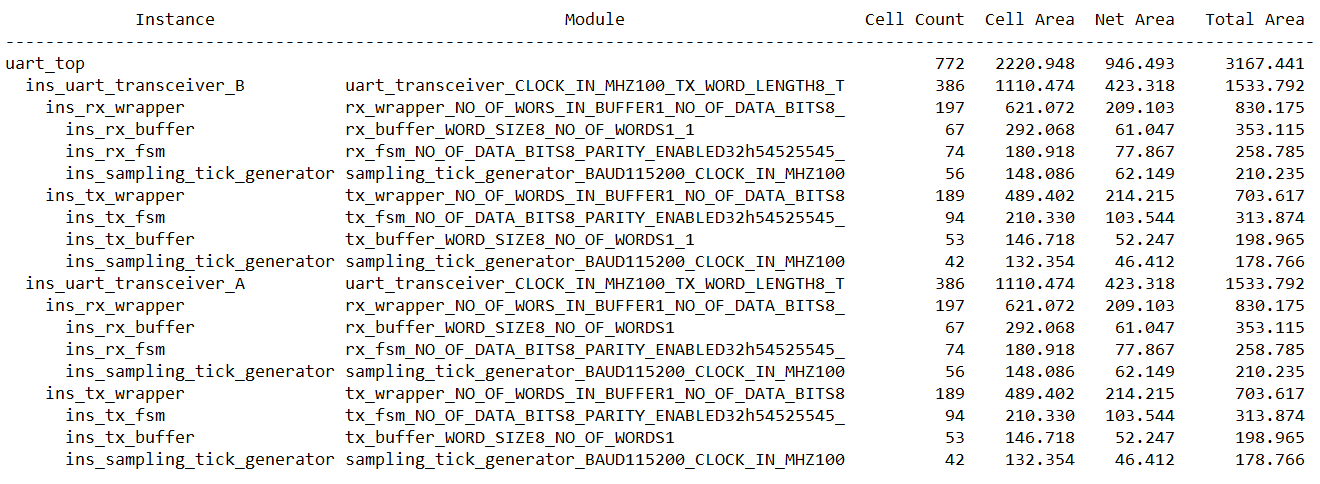
\includegraphics[width=0.95\linewidth]{figures/area_log.PNG}
	}
	\caption{Area log file}
	\label{fig:area_log}
\end{figure}


\subsubsection{Power}
The {\tt power.log} file in the {\tt report} directory carries the details shown in the Figure \ref{fig:power_log}. It provides the information related to the power consumption; however, the returned information depends on the current position in the design hierarchy and on the specified objects. If no objects are specified, the report is given for the design or instance at the current position in the design hierarchy\cite{genus_command_ref_2019}.

\begin{enumerate}[i.] %re check
	\item \textbf{Leakage Power} refers to the power that is consumed by the circuit even when it is in a quiescent or standby state. This type of power consumption is caused by the leakage current flowing through the transistors and other components in the circuit.
	
	\item \textbf{Dynamic Power} refers to the power that is consumed by the circuit when it is actively switching or performing computations. This type of power consumption is caused by the charging and discharging of the load capacitance at the inputs and outputs of the transistors.
	
	\item \textbf{Total Power} is the sum of leakage power and dynamic power, it is the overall power consumed by the circuit.
\end{enumerate}


\begin{figure}[h]
	\centering
	\fbox{
		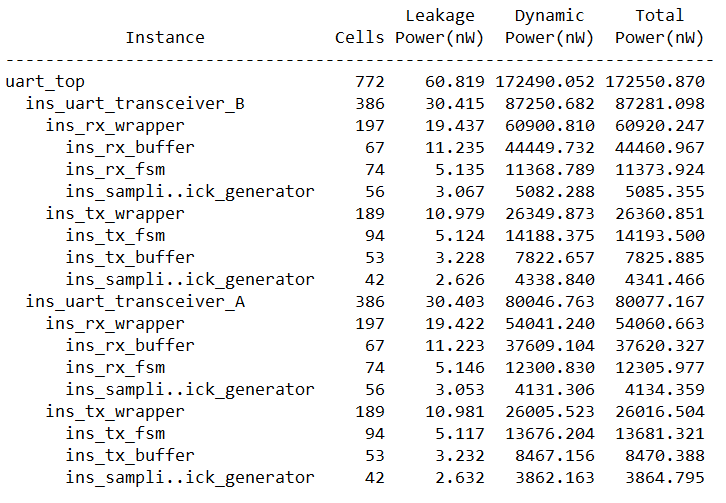
\includegraphics[width=0.75\linewidth]{figures/power_log.PNG}
	}
	\caption{Power log file}
	\label{fig:power_log}
\end{figure}


\subsubsection{Timing}
The {\tt timing.log} file in the {\tt report} directory carries the details shown in the Figure \ref{fig:timing_log}. The command given below was used to generate this timing report. `{\tt -nworst 10}' argument in the command specifies that, the maximum number of paths to report to each endpoint is 10.

\begin{Verbatim}[frame=single]
report_timing  -nworst 10 > ../report/timing.log

Warning : Possible timing problems have been detected in this design. [TIM-11]
: The design is 'uart_top'.
: Use 'report timing -lint' for more information.
\end{Verbatim}

In addition, below constraints are defined in the {\tt constraints.tcl} to be used for the synthesis. Here the input delay is constrained to $6~ns = 6000~ps$, and this information is also available in the timing report shown in the Figure \ref{fig:timing_log}.

\begin{Verbatim}[frame=single]
set_input_delay  6 -clock clk_a  $design_inputs_a
set_input_delay  6 -clock clk_b  $design_inputs_b
set_output_delay 6 -clock clk_a $design_outputs_a
set_output_delay 6 -clock clk_b $design_outputs_b
\end{Verbatim}


\begin{figure}[H]
	\centering
	\fbox{
		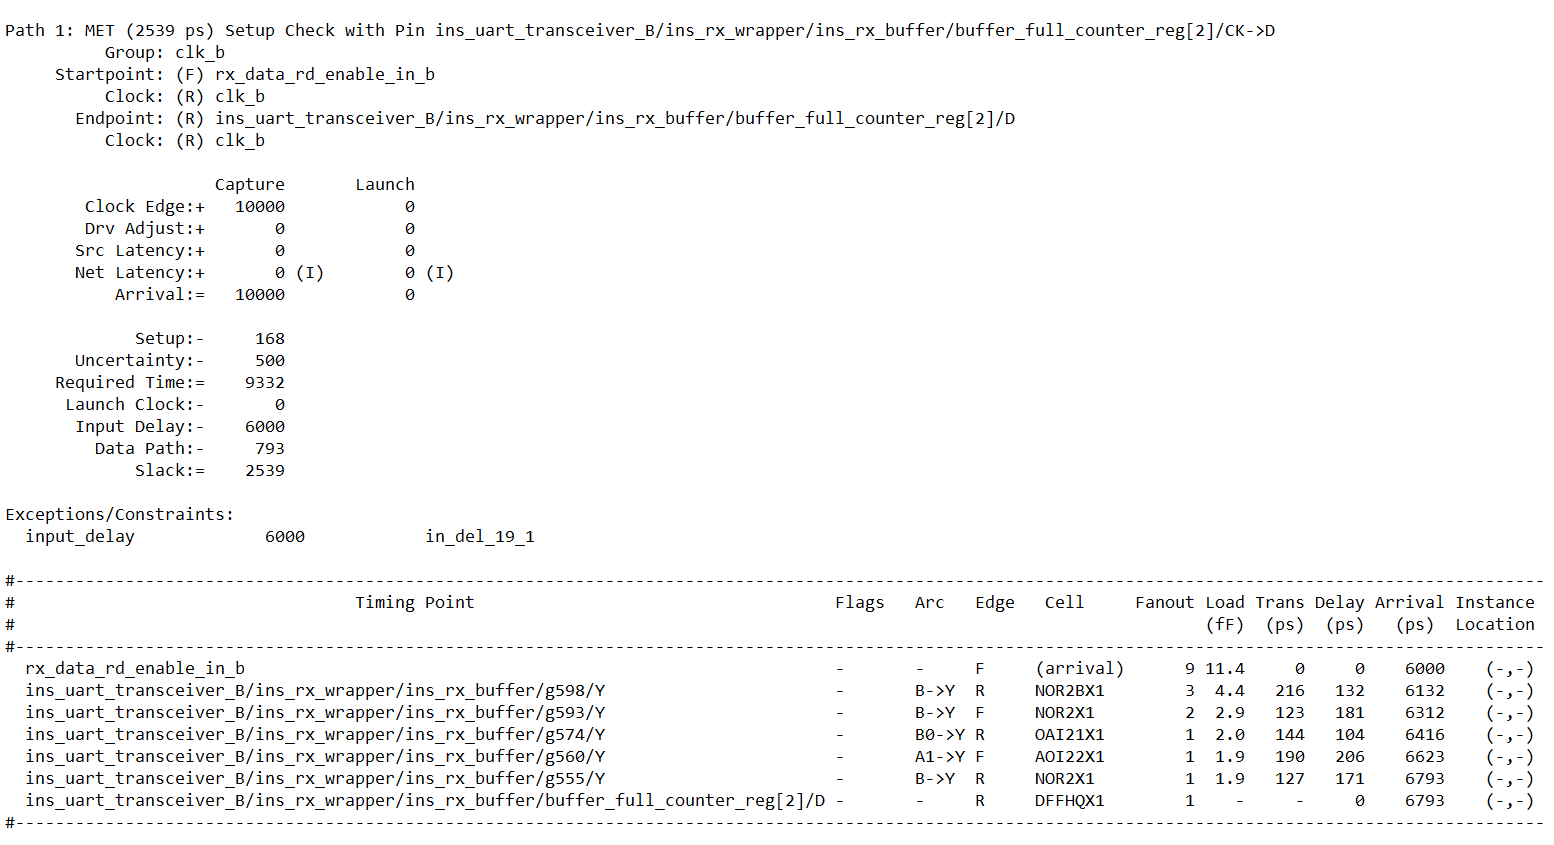
\includegraphics[width=0.95\linewidth]{figures/timing_log.PNG}
	}
	\caption{Timing log file}
	\label{fig:timing_log}
\end{figure}

According to the information found on the timing log file, \textbf{the most critical path} (Path 1 in Figure \ref{fig:timing_log}) has a positive slack time of $2539~ps$.  This is the least slack time of the given design. This indicates that, there is no timing violations in the design.\\

Note: Slack is a measure of the timing margin available in a design. It is the difference between the \textit{Required Time} and the \textit{Arrival Time} of a signal at a specific endpoint. Positive slack indicates that the design meets the timing constraints and there is extra time available, while negative slack indicates that the design does not meet the timing constraints and the path is considered to be in violation. \textbf{The paths with the least slack are the most critical paths}. A design with a high slack value has more margin for manufacturing variations, temperature changes, and other factors that can affect the timing of the system.



\subsubsection{Ports}

\pagebreak
\bibliographystyle{IEEEtran}
\bibliography{refer}

%---------------------------------------------------------------------------
\end{document}
-
